% 
% Annual Cognitive Science Conference
% Sample LaTeX Paper -- Proceedings Format
% 

%% Change "letterpaper" in the following line to "a4paper" if you must.

\documentclass[10pt,letterpaper]{article}

\usepackage{cogsci}
% Recommended, but optional, packages for figures and better typesetting:
\usepackage[margin=1in]{geometry} 
\usepackage{microtype}
\usepackage{graphicx}
\usepackage{subfigure}
\usepackage{booktabs} % for professional tables
\usepackage{nicefrac}       % compact symbols for 1/2f, etc.
\usepackage{microtype}      % microtypography
\usepackage{float}
\usepackage[colorlinks,allcolors=purple]{hyperref}
\usepackage{algorithm}
\usepackage{amsmath}
\usepackage{graphicx}
\usepackage[table,xcdraw]{xcolor}
\usepackage{gensymb}
\usepackage{stmaryrd}
\usepackage{amssymb}

%\cogscifinalcopy % Uncomment this line for the final submission 


\usepackage{pslatex}
\usepackage{apacite}


%\usepackage[none]{hyphenat} % Sometimes it can be useful to turn off
%hyphenation for purposes such as spell checking of the resulting
%PDF.  Uncomment this block to turn off hyphenation.


%\setlength\titlebox{4.5cm}
% You can expand the titlebox if you need extra space
% to show all the authors. Please do not make the titlebox
% smaller than 4.5cm (the original size).
%%If you do, we reserve the right to require you to change it back in
%%the camera-ready version, which could interfere with the timely
%%appearance of your paper in the Proceedings.



\title{Contextually-adapted abstractions explain \\ contextually-adapted abstraction in language} 
 
\author{{\large \bf Morton Ann Gernsbacher (MAG@Macc.Wisc.Edu)} \\
  Department of Psychology, 1202 W. Johnson Street \\
  Madison, WI 53706 USA
  \AND {\large \bf Sharon J.~Derry (SDJ@Macc.Wisc.Edu)} \\
  Department of Educational Psychology, 1025 W. Johnson Street \\
  Madison, WI 53706 USA}


\begin{document}

\maketitle


\begin{abstract}
XXX

\textbf{Keywords:} TBD
\end{abstract}


\section{Introduction} \label{sec-introduction}
\begin{enumerate}
    \item Main question: Language isn’t a monolith -- people can choose many different ways to describe the exact  same thing. What explains that variation in language? Specifically, we focus on grounded language that is about things in the world -- \textbf{what explains the set of concepts people choose to convey that thing, and in particular, what determines the level of abstraction that they choose?}
    \item Prior work (eg. Tian) has demonstrated that people perceive and quickly learn abstract domain structure - in particular, that they are attentive to the set of abstract concepts used to carve up the space, and that the way they parse images drawn from a generative model is consistent with the optimal concept library fit to the stimuli they observe.
    \item We hypothesize that this is reflected in language -- that people produce language that reflects an abstract, domain-specific concept library. 
    \item We adopt the more formal modeling hypothesis in (LOT, Tian, McCarthy, Wong, others): that people represent underlying domain-structure in a compositional, language-like LOT, and specifically, a domain-specific concept library with program-like structure. Therefore, our hypothesis can be evaluated by looking for correlations in the language produced and underlying programs, drawn from differing formal DSLs at different levels of abstraction.
    \item To evaluate this:
        \begin{enumerate}
            \item We collect a corpus of grounded language in which this can be studied systematically in two domains (Section \ref{sec-dataset}), comprised of two domains with hierarchical structure in how the stimuli vary, and permitting multiple levels of abstraction - in which we have access to differing ground truth DSLs that generate the stimuli.
            \item We first compare a base DSL of low-level parts to two increasingly higher order DSLs and find that the language people produce is better explained by a higher-order, part-based concept library (Section B.)

        \end{enumerate}
\end{enumerate}


\begin{figure*}
  \begin{center}
  \includegraphics[width=0.99\linewidth]{figures/task_fig_full.pdf}
  \caption{}
  \label{fig:task}
  \end{center}
  \end{figure*}    

\section{Part I: Domain context influences vocabulary choice} \label{sec-dataset}

Our first goal was to investigate the basic claim that people adapt the set of concepts they use in language -- their vocabulary -- contextually to a given domain. To accomplish this, we design a hierarchical stimuli dataset comprised of images generated by a shared set of basic primitives, but with variation across higher levels of abstraction. We hypothesized that the vocabularies people used to describe these stimuli would be \textit{domain context-specific}: that participants would tend to use different vocabularies tailored to the sub-domain distribution of stimuli they were shown, even when they were generated from the same base primitives. % TODO: 

\subsection{Methods: Language production experiment}



% \begin{enumerate}
%     \item Describe stimuli generation : two domains (gadgets; towers); four subdomains in each.
%     \item Describe language generation task.
% \end{enumerate}
\paragraph{Hierarchical stimulus generation} % two domains (gadgets; towers); four subdomains in each.

% todo: tie to program abstraction
% Desiderata: 1) varied set of categories, 2) hierarchical structure; 3) primitives + higher-order abstractions available to describe, 4) novel + evocative

% 	What do these buy us?
% #1 more general findings
% #2 reminiscent of hierarchical structure of real-world concepts
% #3 allows us to test the notion of "basic-level" but for parts (Rosch et al.) (“just right” level of abstraction)
% #4 lets us look at learning (later)

% 'structures' :  ['bridge', 'castle', 'house', 'city'],
% 'drawing' :  ['nuts-bolts','wheels','furniture','dials']

To investigate how the compositional structure of an object's domain affects the language people use to describe that object, we designed a collection of artificial image stimuli that were hierarchically constructed from smaller parts  (Fig. \ref{fig:task}B).
% Different primitives (i.e. difference between domains)
Our stimulus set consisted of two distinct domains that were each procedurally generated from a set of base primitives.
\textit{Gadgets} were designed to resemble technical drawings of functional objects, and were composed of digital pen strokes.
\textit{Structures} were designed to resemble architectural structures, and were composed of horizontal and vertical blocks.
Each item corresponded to a generative program involving the base primitives of its domain. 
Critically, each domain involved a set of mid-level abstractions  (e.g. \textit{wheels}, \textit{roofs}) that could appear across different stimuli. 

% Different compositional structure within domain (difference between subdomains)
Furthermore, each domain was further subdivided into four subdomains, which were each defined by a distinct generative procedure that was hand-designed to produce objects of a recognizable subordinate category (e.g. \textit{furniture}, \textit{castle}) from a set of predefined abstractions (e.g. \textit{legs}, \textit{tower}).
Several of these abstractions were shared between subdomains (\textit{roofs}, for example appeared in both \textit{houses} and \textit{skyscrapers}), which allowed us to compare the language used to pick out abstraction types in different contexts.
We enumerated all possible stimuli for each subdomain, and selected a random but biased sample of each to obtain 250 stimuli of varying size for each subdomain.


\paragraph{Procedural language production task}

% goal?
% procedural
To evoke a thorough decomposition of each object's component parts, we asked participants to produce a complete sequence of instructions for constructing each stimulus.
Each participant produced instructions for 10 items from a single \textit{subdomain} (e.g. only \textit{castles}), either describing how to ``draw'' the item if describing a subdomain of \textit{gadgets}, or how to ``build'' the item if it was a \textit{structure}.
% what/where framing
To disentangle referring expressions from spatial information, we provided an interface in which participants could enter step-by-step instructions, where each step involved typing \textit{what} would be placed/drawn \textit{where} in separate ``what'' and ``where'' text boxes (Fig. \ref{fig:task}A).
Participants could add as many instruction steps as they liked, and had no time limit.

% familiarization and design
To familiarize participants with the kinds of stimuli and abstraction that could appear in their subdomain, they were first required to click through images of 25 other stimuli from their subdomain, disjoint with the set to be described. 
While describing each image, they could also see up to 7 of the upcoming stimuli.
We collected data from participants until all (2 domains * 4 subdomains * 250) stimuli had been described by at least 2 participants with complete datasets (i.e. had described all 10 of their items).
% \todo{how many participants did we collect in the end? how many descriptions?}
Participants were paid around \$15 per hour for their time. 

\begin{figure*}
  \begin{center}
  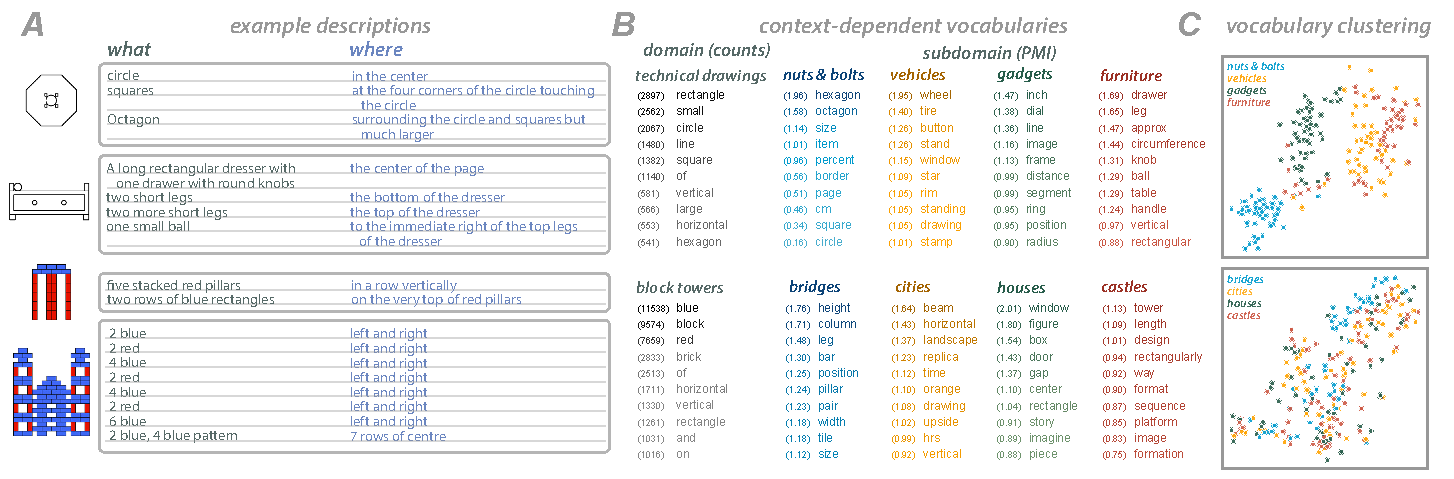
\includegraphics[width=0.99\linewidth]{figures/instruction_examples.pdf}
  \caption{}
  \label{fig:intruction_examples}
  \end{center}
  \end{figure*}

\paragraph{Language preprocessing} % spacy, en_core_web_lg,
To better investigate the content of the instructions generated by participants, we use the spaCy NLP library to extract and lemmatize words. %, as well as remove stop words.

% Add TF-IDF filtering?

% \subsection{People use different words for different domains and subdomains} 

% people use abstractions at all


\subsection{Results}
% ($b=XXX$, $t=XXX$, $p=XXX$)
% $XXX\%$ (95\% CI: $[XXX, XXX]$)

% descriptive statistics of dataset
We collected 4961 sets of instructions from a total of 589 participants. %TK: recalculate
%465 participants completed their set of 10 annotations.
Instructions produced for \textit{castles} tended to be longer than those for \textit{gadgets}, both in terms of the number of instruction steps provided ($b=XXX$, $t=XXX$, $p=XXX$) and the raw character counts ($b=XXX$, $t=XXX$, $p=XXX$).



(Fig. \ref{fig:intruction_examples}).

\par \textbf{Domain-specific abstraction in language}
Our stimuli comprised two domains, each containing items constructed from a set of base primitives.


% histograms

\par \textbf{Subdomain-specific abstraction in language}
We designed our stimuli to break into several subdomains containing different abstractions over the base primitives used to construct items in the domain.
Did the instructions produced by participants reflect these differences in subdomain structure?

% histograms

\section{Part II: Language complexity correlates non-linearly with base primitive complexity} \label{sec-part-ii}

Our language production experiment and initial vocabulary analysis established that people use words that are contextually-adapted to the domain.

However, the stimuli across each domain are generated using a shared set of base primitives -- all structures are generated using the same procedural programs that place primitive \textit{blocks}, and all drawings are generated by transformations over a set of primitive \textit{strokes}. Before considering more abstract representations, we can first ask: how well do these base primitive representations explain language production? We conducted a control experiment to establish an initial correspondence between the procedural program representations of each stimulus in the base DSL and language, by correlating token length in the base DSL with token length in language.

We hypothesized that there would be a positive, but non-linear, correlation between base DSL description length and human language: we expect that even when measured in low-level primitives, more complex stimuli should require more words to describe; but we also expect that the existence of domain-specific abstractions named in language (as established in Section I) should mean that people's language length should not scale linearly with the number of blocks or strokes in each stimulus.

% Why is there variance in instruction length?
% Variance in complexity

% But complexity doesn't explain everything-- in fact people are able to condense complex items into condensed abstractions. And this is borne out by a non-linear relationship between task complexity and instruction length.
% Explain handcoded abstractions

% Library size? 


\section{Part III: Contextually-adapted abstractions can better predict language production}
Our results so far suggest that people use contextually-adapted vocabularies to describe stimuli (Part I); and that the lowest-level, base primitive representation of each object only partially explains the words a person needs to describe it -- in particular, people are often able to describe an object using fewer words than the base primitive representation would predict (Part II). Taken together, an intuitive explanation for these results is that -- while a person could in principle use the exact same vocabulary of low-level base concepts to describe any given stimulus in the domain -- they instead choose to compose words that reflect a vocabulary of higher-level, context-specific abstractions adapted to the specific distribution of stimuli they were asked to describe.

Here, we present a formal method for evaluating the specific set of abstractions, and the level of abstractions, people use in language. Concretely, we generate context-specific DSLs at varying levels of abstraction for each subdomain, which add increasingly high-level, context-specific abstractions to the initial set of base primitives. We then re-represent each stimulus under these varying levels of program abstraction, and 

vary the level of abstraction in the generative programs for each subdomain by adding in increasingly high-level, but context-specific, program abstractions to the initial set of base primitives. We then fit a program-language preidction model to each  


Here, we present a formal method for evaluating both the level of abstraction and the specific set of abstractions people use in language. Concretely, we re-represent the generative programs for each subdomain under varying levels of parametric abstraction, and then compare how well programs at each level can be used to explain human language using a formal program-language prediction model fit to each subdomain. We first hypothesize that 

However, this formal . We therefore more specifically hypothesize that an \textit{intermediate} level of contextual abstraction, determined formally by the DSL complexity, should best predict language in each subdomain: 


\subsection{Methods: Identifying language abstraction with varying levels of program abstraction}
The results so far show that 

\paragraph{Generating multiple levels of program abstractions} How we generated DSLs.
\paragraph{Correlating program abstractions with language} Translation models.

\begin{figure*}
  \begin{center}
  \includegraphics[width=0.99\linewidth]{figures/fig_language_libraries.pdf}
  \caption{}
  \label{fig:lanuage_libraries}
  \end{center}
  \end{figure*}
  



\section{Discussion}

% How contextual is the level of abstraction? 
%   => Collect more data for item-specific and speaker-specific variation
%   => Modulate size of domain even more

% How do communicative goals modulate the ‘right’ level/ kind of abstraction?
%   => Other contexts e.g. reference-games
  
% How does individual learning modulate speaker-specific abstraction?
%   =>  Pre-post study: individual non-linguistic experience vs. individual language usage
  
% How does shared experience modulate the level of abstraction?
%   => Paired tasks (CA++)

\bibliographystyle{apacite}

\setlength{\bibleftmargin}{.125in}
\setlength{\bibindent}{-\bibleftmargin}

\bibliography{CogSci_Template}


\end{document}
